\documentclass[a4paper,12pt]{article}

\usepackage{graphicx}
\usepackage{hyperref}
\graphicspath{{images/}}
\begin{document}

\section{Use Case: Template Messaging}
This use case deals with using templates to send messages to individuals as well as groups of users. A user with a high enough privilege will be able to send messages directly to other users. The messages may be formatted with a template of choice.

\subsection{Use Case Prioritization}
This feature of the forum is not critical but it is important. Administrators of the forum must be able to directly communicate with users to issue warnings or give out help and advice.

\subsection{Service Contracts}
Pre-conditions: 
\begin{itemize}
\item The user must have the required privileges/level
\item The database must be online
\item Recipients must be registered users
\end{itemize}
      
Post-Conditions:
\begin{itemize}
\item Recipients have received their messages
\item Message(s) successfully sent
\end{itemize}
      
\subsection{Process}
Once a user has the required privileges he/she will be able to send messages to other users. Upon using the service, the user will be asked to type out the message he/she wishes to send. Next the template and format of the message will be chosen. Finally the Recipient(s) of the message will be specified with the aid of the search function. 

\subsection{Use Case Diagram}
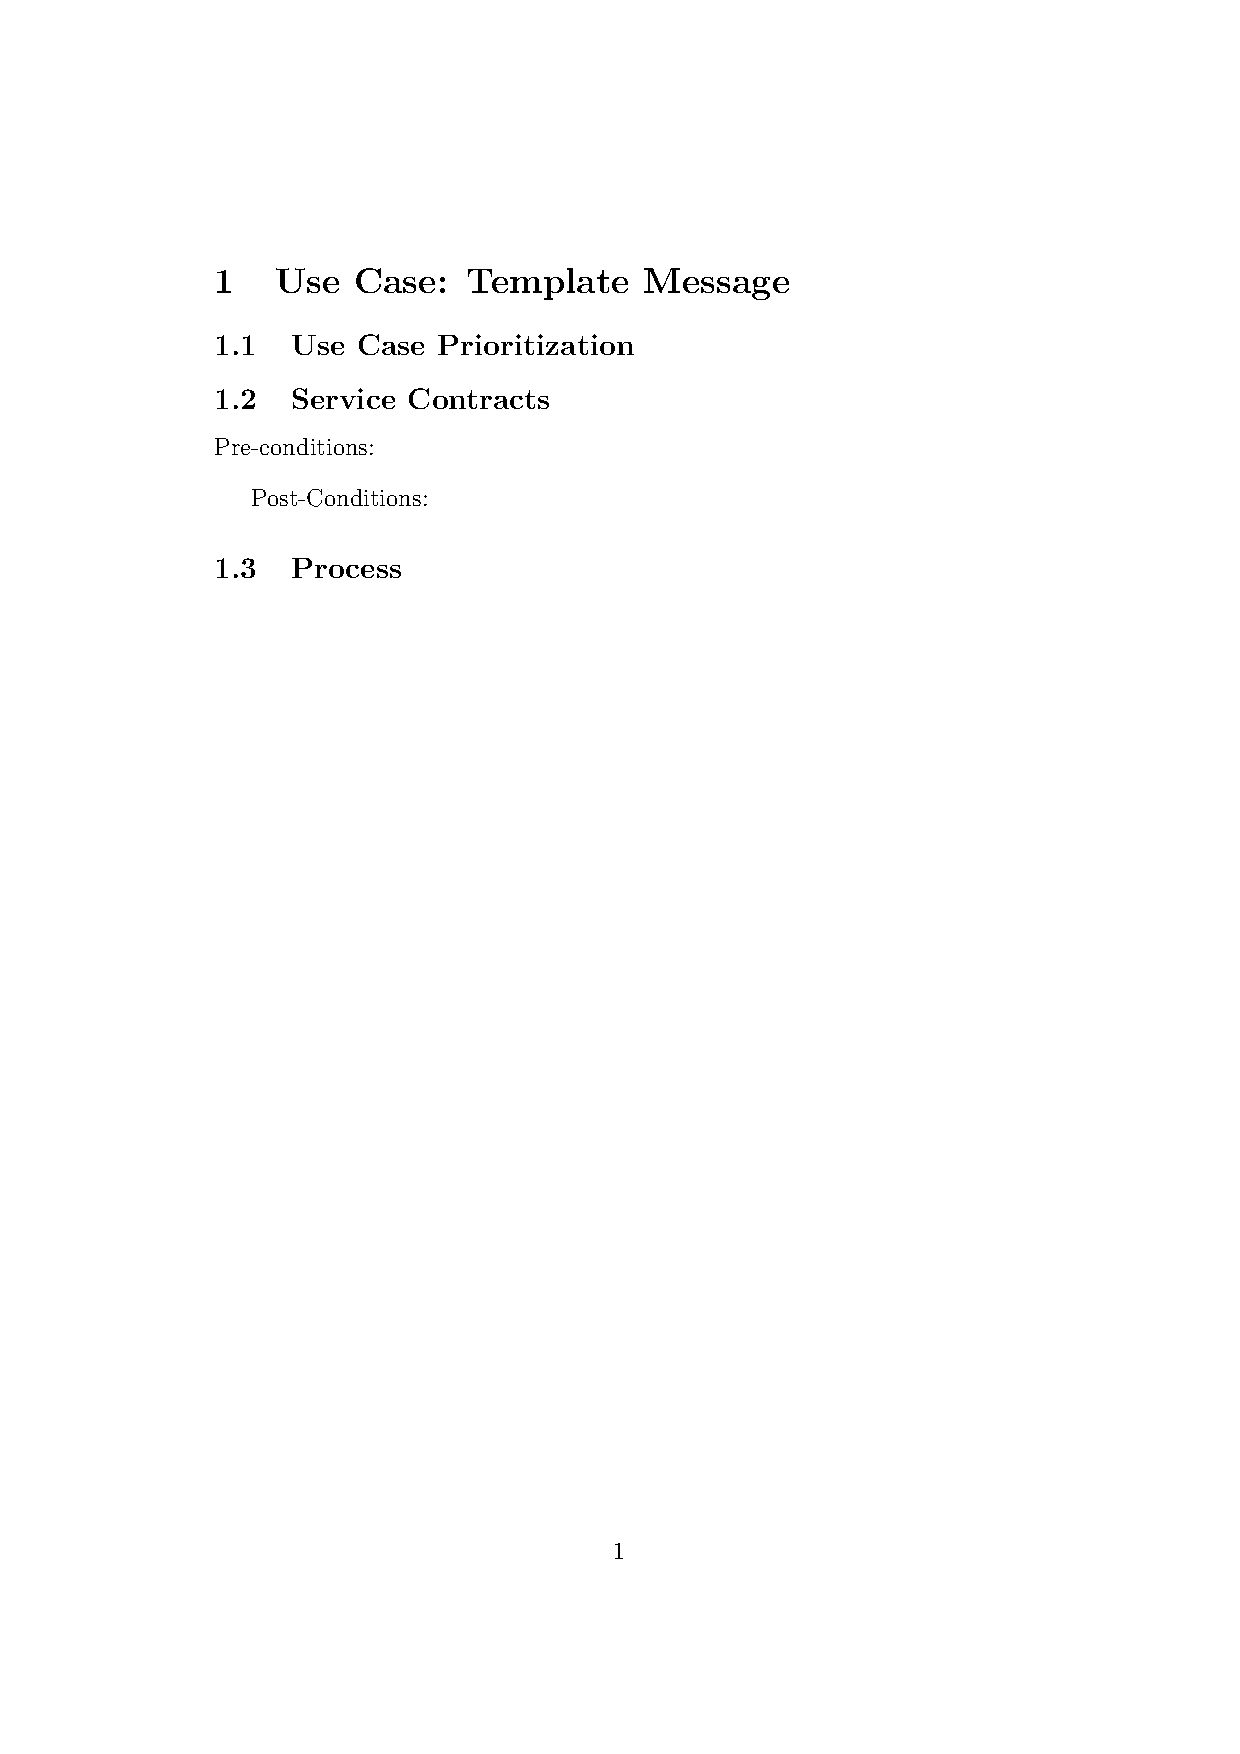
\includegraphics{12260429_TemplateMessaging}

\end{document}
